\documentclass[aspectratio=169]{beamer}

\definecolor{red}{RGB}{220, 50, 47}
\definecolor{green}{RGB}{133, 153, 0}
\definecolor{cyan}{RGB}{42, 161, 152}
\definecolor{blue}{RGB}{38, 139, 210}
\definecolor{yellow}{RGB}{181, 137, 0}

% Suppress all navigation symbols
\setbeamertemplate{navigation symbols}{}
\setbeamertemplate{headline}{}
\setbeamertemplate{footline}{}
\setbeamertemplate{itemize items}[circle]
\setbeamertemplate{footline}[frame number]

\setbeamercolor{structure}{fg=blue}
\setbeamercolor{normal text}{fg=black, bg=white}
\setbeamerfont{title}{series=\bfseries}
\setbeamerfont{frametitle}{series=\bfseries}

\setbeamertemplate{footline}{
  \begin{tikzpicture}[remember picture,
                      overlay,
                      shift={(current page.south west)}]
    \node [black!50, inner sep=2mm, anchor=south east] at (current page.south east) {\large \bfseries \insertframenumber};
  \end{tikzpicture}
}

\usepackage{fontspec}
\setmainfont[Ligatures=TeX]{Tinos}
\setsansfont{Arimo}[Scale=MatchLowercase]
\setmonofont{Cousine}[Scale=MatchLowercase]

\usepackage{tikz}
\usetikzlibrary{arrows}
\usetikzlibrary{calc}
\usetikzlibrary{decorations.pathreplacing}
\usetikzlibrary{positioning}
\usetikzlibrary{matrix}
\usetikzlibrary{shapes}

\title{C++ const and Immutability: An Empirical Study of
       Writes-Through-const}
\author{Jon Eyolfson}
\date{2016-07-20}

\newcommand{\const}{{\color{blue} \bfseries \ttfamily const}}

\setbeamertemplate{title page}
{
  \begin{tikzpicture}[remember picture,
                      overlay,
                      shift={(current page.south west)}]
    \node (title) [inner sep=0, scale=1.5, align=left]
          at (\paperwidth / 2, \paperheight * 2 / 3)
          {\usebeamerfont{title}\usebeamercolor[fg]{title}C++ \const{} and
           \usebeamerfont{title}\usebeamercolor[fg]{title}Immutability:\\
           \usebeamerfont{title}\usebeamercolor[fg]{title}An Empirical
           \usebeamerfont{title}\usebeamercolor[fg]{title}Study of Writes-Through-\const{}};

    \node (author) [scale=1.5] at (\paperwidth / 3, \paperheight / 3) {\insertauthor};
    \node [node distance=-2mm, below=of author] {\texttt{https://eyl.io/}};
    \node (a2) [scale=1.5] at (\paperwidth * 2 / 3, \paperheight / 3) {Patrick Lam};
    \node [node distance=-2mm, below=of a2] {\texttt{https://patricklam.ca/}};
    \node [anchor=south east] at (\paperwidth, 0) {\insertdate};
    \node [yshift=-2mm] at (\paperwidth / 2, \paperheight /2) {\includegraphics[scale=0.3]{uwaterloo-logo}};
  \end{tikzpicture}
}

\newlength{\barlength}
\setlength{\barlength}{10cm}

\newcommand{\transition}[1]{
  \begin{frame}
    \begin{center}
      \usebeamerfont{title}\usebeamercolor[fg]{title}#1
    \end{center}
  \end{frame}
}

\tikzset{
  every matrix/.style={
    fill=black!20,
    inner sep=2mm, row sep=0.5mm,
    matrix of nodes, nodes in empty cells,
    minimum height=0.5em, minimum width=.75em,
    nodes={anchor=base, inner sep=0, font=\ttfamily},
    ampersand replacement=\&
  },
  arrow/.style={->,>=stealth',shorten >=1mm, shorten <=1mm, thick}
}

\begin{document}

  \begin{frame}[plain]
    \titlepage
  \end{frame}

  \setcounter{framenumber}{0}

  \begin{frame}
    \frametitle{Immutability}
    \centering
    \begin{tikzpicture}[remember picture,
                        overlay,
                        shift={(current page.south west)}]
      \node [align=center, font=\huge] at (\paperwidth / 3, \paperheight / 2)
            {\bfseries Conceptually:\\``things''\\do not\\``change''};
      \node at (\paperwidth * 2 / 3, \paperheight / 2) [draw=red, line width=3mm, forbidden sign, font=\Huge,
             minimum size=20mm]
        {\bfseries Change};
    \end{tikzpicture}
  \end{frame}

  \begin{frame}
    \frametitle{Two ``Things'' of Immutability}
    \Large
    \begin{tikzpicture}[remember picture,
                        overlay,
                        shift={(current page.south west)}]
      \tikzset{memory/.style={draw, rectangle, node distance=0,
                              line width=0.3mm, scale=1.25,
                              minimum height=8mm, minimum width=6mm}}
      \node [inner sep=0, scale=1.25, yshift=4mm] (o)
            at (\paperwidth / 5, \paperheight * 2 / 3)
            {Object \texttt{o}};
      \node [memory, right=of o, xshift=3mm] (f0)
            {$f_x$};
      \node [memory, right=of f0, xshift=-0.3mm] (f1) {$f_y$};
      \node [node distance=0, right=of f1, xshift=-0.3mm] (dots) {$...$};
      \node [memory, right=of dots, xshift=-0.3mm] (fn) {$f_z$};

      \node [memory, below=of f0, xshift=-15mm, yshift=-15mm] (m0) {};

      \node [memory, below=of fn, yshift=-15mm] (mn) {};

      \node [memory, below=of m0, xshift=12mm, yshift=-6mm] (t0) {};

      \node at (o.west)
            [xshift=-3mm, draw, line width=0.3mm, minimum width=58mm,
             minimum height=12mm, anchor=west] {};

      \node at (f0.west)
           [anchor=west, xshift=-1mm, fill opacity=0.5, text opacity=1,
            fill=yellow, align=right,
            minimum height=12mm, text width=95mm]
           {Shallow immutability boundary};

      \node at (m0.west)
           [anchor=west, xshift=-1mm, fill opacity=0.5, text opacity=1,
            fill=yellow, align=right, yshift=-9mm,
            minimum height=30mm, text width=113.5mm]
           {Deep immutability boundary};

      \path[arrow] (f0) edge [bend left] (m0)
                   (fn) edge (mn)
                   (m0) edge [bend left] (t0);
    \end{tikzpicture}
  \end{frame}

  \begin{frame}
    \frametitle{Two ``Changes'' of Immutability}
    \Large
    Bitwise: no writes
 
    \vspace{1em}
    Logically: no observable changes
  \end{frame}

  \begin{frame}
    \frametitle{C++ \const{} and Immutability}
    \Large
    C++ has a \const{} type qualifier for developers to specify immutability

    \vspace{1em}
    Without escape hatches: \structure{shallow bitwise} immutable

    \vspace{1em}
    With escape hatches: (possibly) \structure{shallow logically} immutable
  \end{frame}

  \begin{frame}
    \frametitle{\const{} Without Escape Hatches}
    \Large
    \structure{Shallow bitwise} immutable

    \vspace{1em}
    No writes to fields within \const{} qualified methods

    \vspace{1em}
    \centering
    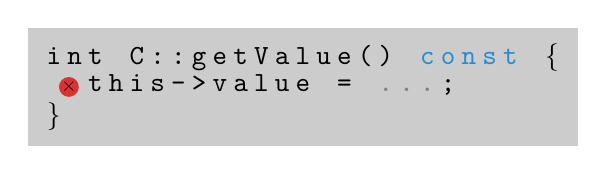
\begin{tikzpicture}
      \matrix (bad) {
        i \& n \& t \&   \& C \& : \& : \& g \& e \& t \& V \& a \& l \& u \&
        e \& ( \& ) \&   \& |[blue]|c \& |[blue]|o \& |[blue]|n \& |[blue]|s \&
        |[blue]|t \& \& \{ \\


        \& \& t \& h \& i \& s \& - \& > \& v \& a \& l \& u \& e \& \& = \&
        \& |[black!50]|. \& |[black!50]|. \& |[black!50]|. \& ; \\

        \} \\
      };
      \node [right=of bad.west, inner sep=0, xshift=-6mm, circle, fill=red,
             scale=0.7]
            {$\times$};
    \end{tikzpicture}
  \end{frame}

  \begin{frame}
    \frametitle{\const{} With Escape Hatches}
    \Large
    Allows \structure{shallow logically} immutable

    \vspace{1em}
    Writes to fields (declared \texttt{mutable}) within \const{} qualified methods

    \vspace{1em}
    \centering
    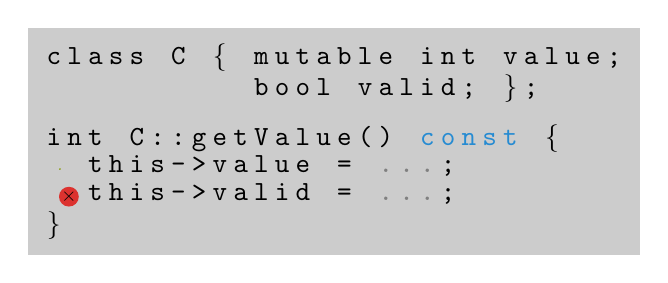
\begin{tikzpicture}
      \matrix (bad) {
        c \& l \& a \& s \&s \& \& C \& \& \{ \& \& m \& u \& t \& a \& b \& l \& e \& \& i \& n \& t \& \& v \& a
        \& l \& u \& e \& ; \\

        \& \& \& \& \& \& \& \& \& \& b \& o \& o \& l \& \& v \& a
        \& l \& i \& d \& ; \& \& \} \& ; \\

        \\


        i \& n \& t \&   \& C \& : \& : \& g \& e \& t \& V \& a \& l \& u \&
        e \& ( \& ) \&   \& |[blue]|c \& |[blue]|o \& |[blue]|n \& |[blue]|s \&
        |[blue]|t \& \& \{ \\


        \& \& t \& h \& i \& s \& - \& > \& v \& a \& l \& u \& e \& \& = \&
        \& |[black!50]|. \& |[black!50]|. \& |[black!50]|. \& ; \\

        \& \& t \& h \& i \& s \& - \& > \& v \& a \& l \& i \& d \& \& = \&
        \& |[black!50]|. \& |[black!50]|. \& |[black!50]|. \& ; \\

        \} \\
      };
      \node [right=of bad.west, inner sep=0, xshift=-6mm, yshift=-1em, circle,
             fill=green, scale=0.7]
            {$\checkmark$};
      \node [right=of bad.west, inner sep=0, xshift=-6mm, yshift=-2em, circle,
             fill=red, scale=0.7]
            {$\times$};
    \end{tikzpicture}
  \end{frame}

  \begin{frame}
    \frametitle{Calling a \const{} Method Does Not Change the Object}
    \large
    \centering
    \begin{tikzpicture}[remember picture,
                        overlay,
                        shift={(current page.south west)}]
      \matrix (decl) at ($ (current page.center) + (0, 25mm) $) {
        i \& n \& t \&   \& C \& : \& : \& g \& e \& t \& V \& a \& l \& u \&
        e \& ( \& ) \&   \& |[blue]|c \& |[blue]|o \& |[blue]|n \& |[blue]|s \&
        |[blue]|t \& ; \\
      };
    \end{tikzpicture}
  \end{frame}

  \begin{frame}
    \frametitle{Example of Shallow Bitwise Immutable}
    \centering
    \large
    \begin{tikzpicture}[remember picture,
                        overlay,
                        shift={(current page.south west)}]

      \matrix (decl) at ($ (current page.center) + (0, 25mm) $) {
        i \& n \& t \&   \& C \& : \& : \& g \& e \& t \& V \& a \& l \& u \&
        e \& ( \& ) \&   \& |[blue]|c \& |[blue]|o \& |[blue]|n \& |[blue]|s \&
        |[blue]|t \& ; \\
      };


      \matrix (defn) [below=of decl] {
        i \& n \& t \&   \& C \& : \& : \& g \& e \& t \& V \& a \& l \& u \&
        e \& ( \& ) \&   \& |[blue]|c \& |[blue]|o \& |[blue]|n \& |[blue]|s
        \& |[blue]|t \&   \& \{ \& \& \\

  \&   \& r \& e \& t \& u \& r \& n \&   \& l \& o \& n \& g \& C \& a \& l \& c \& u \& l \& a \& t \& i \& o \& n \& ( \& ) \& ; \\
\} \&   \&   \&   \&   \&   \&   \&   \&   \&   \&   \&   \&   \&   \&   \&   \&   \&   \&   \&   \&   \&   \&   \&   \&   \&   \&   \\
  };

      \draw [arrow] (decl) -- node [right, xshift=1mm] {\normalsize Slow} (defn);
    \end{tikzpicture}
  \end{frame}

  \begin{frame}
    \frametitle{Example of Shallow Logically Immutable}
    \large
    \centering
    \begin{tikzpicture}[remember picture,
                        overlay,
                        shift={(current page.south west)}]
      \matrix (decl) at ($ (current page.center) + (0, 25mm) $) {
        i \& n \& t \&   \& C \& : \& : \& g \& e \& t \& V \& a \& l \& u \&
        e \& ( \& ) \&   \& |[blue]|c \& |[blue]|o \& |[blue]|n \& |[blue]|s \&
        |[blue]|t \& ; \\
      };

      \matrix (defn) [below=of decl] {
        c \& l \& a \& s \&s \& \& C \& \& \{ \& \& m \& u \& t \& a \& b \& l \& e \& \& i \& n \& t \& \& v \& a
        \& l \& u \& e \& ; \\

        \& \& \& \& \& \& \& \& \& \& m \& u \& t \& a \& b \& l \& e \& \& b \& o \& o \& l \& \& v \& a
        \& l \& i \& d \& ; \& \& \} \& ; \\

        \\

        i \& n \& t \&   \& C \& : \& : \& g \& e \& t \& V \& a \& l \& u \& e \& ( \& ) \&   \& |[blue]|c \& |[blue]|o \& |[blue]|n \& |[blue]|s \& |[blue]|t \&   \& \{ \\

  \&   \& i \& f \&   \& ( \& ! \& |[black!50]|t \& |[black!50]|h \& |[black!50]|i \& |[black!50]|s \& |[black!50]|- \& |[black!50]|> \& v \& a \& l \& i \& d \& ) \&   \& \{ \\

  \&   \&   \&   \& |[black!50]|t \& |[black!50]|h \& |[black!50]|i \& |[black!50]|s \& |[black!50]|- \& |[black!50]|> \& v \& a \& l \& u \& e \&   \& = \&   \& l \& o \& n \& g \& C \& a \& l \& c \& u \& l \& a \& t \& i \& o \& n \& ( \& ) \& ; \\

  \&   \&   \&   \& |[black!50]|t \& |[black!50]|h \& |[black!50]|i \& |[black!50]|s \& |[black!50]|- \& |[black!50]|> \& v \& a \& l \& i \& d \&   \& = \&   \& t \& r \& u \& e \& ; \\

      \&   \& \} \\

  \&   \& r \& e \& t \& u \& r \& n \&   \& |[black!50]|t \& |[black!50]|h \& |[black!50]|i \& |[black!50]|s \& |[black!50]|- \& |[black!50]|> \& v \& a \& l \& u \& e \& ; \\

        \} \\
      };
      \draw [arrow] (decl) -- node [right, xshift=1mm] {\normalsize Fast} (defn);
    \end{tikzpicture}
  \end{frame}

  \begin{frame}
    \frametitle{Incorrect \const{} Methods Lead to Issues}
    \large
    \centering
    \begin{tikzpicture}[remember picture,
                        overlay,
                        shift={(current page.south west)},
                        node distance=5mm]
      \matrix (unrelated) at ($ (current page.center) + (0, 21mm) $) {
v \& o \& i \& d \&   \& C \& : \& : \& u \& n \& r \& e \& l \& a \& t \& e \& d \& ( \& ) \&   \& |[blue]|c \& |
[blue]|o \& |[blue]|n \& |[blue]|s \& |[blue]|t \& \& \{ \\

        \& \& t \& h \& i \& s \& - \& > \& v \& a \& l \& u \& e \& \& = \&
        \& 4 \& 2 \& ; \\

        \} \\
      };

      \matrix (first) [node distance=16mm, below=of unrelated, minimum width=40mm] {
        \& |[blue]|c \& |[blue]|o \& |[blue]|n \& |[blue]|s \& |[blue]|t \& \& C
        \&  \& c \& ; \\

        \& u \& n \& o \& r \& d \& e \& r \& e \& d \& \_ \& m \& a \& p \& . \& f \& i \& n \& d \& ( \& c \& ) \& ; \\

        \& c \& . \& u \& n \& r \& e \& l \& a \& t \& e \& d \& ( \& ) \& ; \& \& \& \& \& \& \& \& \\

        \& u \& n \& o \& r \& d \& e \& r \& e \& d \& \_ \& m \& a \& p \& . \& f \& i \& n \& d \& ( \& c \& ) \& ; \\
      };

      \node at (current page.center) {\normalsize Assume \texttt{getValue()} used as hash};

      \node [right=of first.west, inner sep=0, xshift=-4mm, yshift=0.75em, circle,
             fill=green, scale=0.7]
            {$\checkmark$};

      \node [right=of first.west, inner sep=0, xshift=-4mm, yshift=-1.5em, circle,
             fill=red, scale=0.7]
            {$\times$};

    \end{tikzpicture}
  \end{frame}

  \begin{frame}
    \frametitle{C++ Does Not Prevent Deep Bitwise Immutability}
    \large
    \centering
    \begin{tikzpicture}[remember picture,
                        overlay,
                        shift={(current page.south west)}]
      \matrix (decl) at ($ (current page.center) + (0, 25mm) $) {
        i \& n \& t \&   \& C \& : \& : \& g \& e \& t \& V \& a \& l \& u \&
        e \& ( \& ) \&   \& |[blue]|c \& |[blue]|o \& |[blue]|n \& |[blue]|s \&
        |[blue]|t \& ; \\
      };

      \matrix (defn) [below=of decl] {
        c \& l \& a \& s \&s \& \& C \& \& \{ \& \& i \& n \& t \& \& * \& \& v \& a
        \& l \& u \& e \& ; \\

        \& \& \& \& \& \& \& \& \& \& b \& o \& o \& l \& \& * \& \& v \& a
        \& l \& i \& d \& ; \& \& \} \& ; \\

        \\

        i \& n \& t \&   \& C \& : \& : \& g \& e \& t \& V \& a \& l \& u \& e \& ( \& ) \&   \& |[blue]|c \& |[blue]|o \& |[blue]|n \& |[blue]|s \& |[blue]|t \&   \& \{ \\

  \&   \& i \& f \&   \& ( \& ! \& * \& ( \& |[black!50]|t \& |[black!50]|h \& |[black!50]|i \& |[black!50]|s \& |[black!50]|- \& |[black!50]|> \& v \& a \& l \& i \& d \& ) \& ) \&   \& \{ \\

  \&   \&   \&   \& * \& ( \& |[black!50]|t \& |[black!50]|h \& |[black!50]|i \& |[black!50]|s \& |[black!50]|- \& |[black!50]|> \& v \& a \& l \& u \& e \& ) \& \& = \&   \& l \& o \& n \& g \& C \& a \& l \& c \& u \& l \& a \& t \& i \& o \& n \& ( \& ) \& ; \\

  \&   \&   \&   \& * \& ( \& |[black!50]|t \& |[black!50]|h \& |[black!50]|i \& |[black!50]|s \& |[black!50]|- \& |[black!50]|> \& v \& a \& l \& i \& d \& ) \& \& = \&   \& t \& r \& u \& e \& ; \\

      \&   \& \} \\

  \&   \& r \& e \& t \& u \& r \& n \&   \& * \& ( \&|[black!50]|t \& |[black!50]|h \& |[black!50]|i \& |[black!50]|s \& |[black!50]|- \& |[black!50]|> \& v \& a \& l \& u \& e \& ) \& ; \\

        \} \\
      };
      \draw [arrow] (decl) -- node [right, xshift=1mm] {\normalsize Fast (without \texttt{mutable})} (defn);
    \end{tikzpicture}
  \end{frame}


  \begin{frame}
    \frametitle{Does \const{} Mean Deep Logically Immutable?}
    \Large

    Our analysis applies \const{} through fields transitively
    \\(i.e. deep immutability)

    \vspace{1em}
    Report any \structure{deep bitwise} immutable violations at runtime
    \\(referred to as writes-through-\const{})

    \vspace{1em}
    Manually classify writes-through-\const{} as \structure{logically} immutable
    or not
  \end{frame}

  \begin{frame}
    \Large
    {\usebeamerfont{title}\usebeamercolor[fg]{title}
     Research Question 1: Do developers write-though-\const{}?}

    \vspace{1em}
    Yes, they do
  \end{frame}

  \begin{frame}
    \Large
    {\usebeamerfont{title}\usebeamercolor[fg]{title}
     Research Question 2: How developers write-though-\const{}?}

    \vspace{1em}
    Equally shallow (using \texttt{mutable}) and deep (transitively)
  \end{frame}

  \begin{frame}
    \Large
    {\usebeamerfont{title}\usebeamercolor[fg]{title}
     Research Question 3: Why do developers write-though-\const{}?}

    \vspace{1em}
    Conventional wisdom: buffering / caching

    \vspace{1em}
    Found \structure{around half} had observable changes (invalid)
  \end{frame}

  \begin{frame}
    \frametitle{Our Dynamic Analysis Reports Writes-Through-\const{}}
    \Large
    Based on the sanitizer family of Clang tools --- ConstSanitizer

    \vspace{1em}
    Adds instrumentation during compilation

    \vspace{1em}
    Linking includes our runtime library that reports writes
  \end{frame}

  % In the case where developer intent is a maybe, we assume they did NOT mean const

  \begin{frame}
    \frametitle{Instrumentation Adds Shadow Values for Variables}
    \Large
    Shadow value encode \const{} qualifiers based on type \texttt{T}

    \centering
    \vspace{2em}
    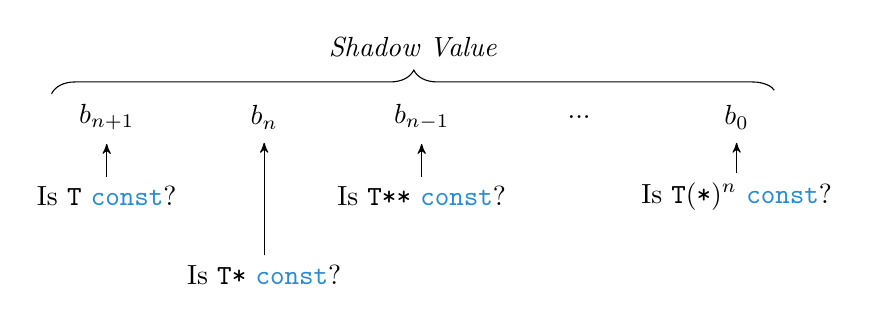
\begin{tikzpicture}[->,>=stealth',shorten >=0.5mm,node distance=2cm]

    \draw [decorate,decoration={brace,amplitude=3mm},-,xshift=0pt,yshift=0pt]
          (-0.7,0.3) -- (8.5,0.3)node [black,midway,yshift=0.6cm]
          {\textit{Shadow Value}};
    \node (b1) {$b_{n+1}$};
    \node [right of=b1] (b2) {$b_n$};
    \node [right of=b2] (b3) {$b_{n-1}$};
    \node [right of=b3] (b4) {...};
    \node [right of=b4] (b5) {$b_0$};
    \node [below of=b1, node distance=1cm] (b1t)
          {Is \texttt{T} \const{}?};
    \node [below of=b2] (b2t)
          {Is \texttt{T*} \const{}?};
    \node [below of=b3, node distance=1cm] (b3t)
          {Is \texttt{T**} \const{}?};
    \node [below of=b5, node distance=1cm] (b5t)
          {Is \texttt{T$(\texttt{*})^n$} \const{}?};

    \path (b1t) edge (b1)
          (b2t) edge (b2)
          (b3t) edge (b3)
          (b5t) edge (b5);
    \end{tikzpicture}
  \end{frame}

  \begin{frame}
    \frametitle{Our Shadow Values Propagate \const{}}
    \large
    \begin{tikzpicture}[remember picture,
                        overlay,
                        shift={(current page.south west)}]
      \matrix (defn) at ($ (current page.center) - (20mm, 10mm) $) {
        i \& n \& t \&   \& C \& : \& : \& g \& e \& t \& V \& a \& l \& u \& e \& ( \& ) \&   \& |[blue]|c \& |[blue]|o \& |[blue]|n \& |[blue]|s \& |[blue]|t \&   \& \{ \\

  \&   \& i \& f \&  \& ( \& ! \& |[black!50]|t \& |[black!50]|h \& |[black!50]|i \& |[black!50]|s \& |[black!50]|- \& |[black!50]|> \& i \& s \& \_ \& c \& a \& c \& h \& e \& \_ \& v \& a \& l \& i \& d \& ) \&   \& \{  \\

  \&   \&   \&   \& |[black!50]|t \& |[black!50]|h \& |[black!50]|i \& |[black!50]|s \& |[black!50]|- \& |[black!50]|> \& c \& a \& c \& h \& e \& d \& \_ \& v \& a \& l \& u \& e \&   \& = \&   \& |[black!50]|. \& |[black!50]|. \& |[black!50]|. \& ; \\

  \&   \&   \&   \& |[black!50]|t \& |[black!50]|h \& |[black!50]|i \& |[black!50]|s \& |[black!50]|- \& |[black!50]|> \& i \& s \& \_ \& c \& a \& c \& h \& e \& \_ \& v \& a \& l \& i \& d \&   \& = \&   \& |[black!50]|. \& |[black!50]|. \& |[black!50]|. \& ; \\

        \& \& \} \\

  \&   \& r \& e \& t \& u \& r \& n \&   \& |[black!50]|t \& |[black!50]|h \& |[black!50]|i \& |[black!50]|s \& |[black!50]|- \& |[black!50]|> \& c \& a \& c \& h \& e \& d \& \_ \& v \& a \& l \& u \& e \& ; \\

        \} \\
      };

      \matrix (call) [above=of defn] {
        |[blue]|c \& |[blue]|o \& |[blue]|n \& |[blue]|s \& |[blue]|t \& \& C
        \&  \& c \& ; \\

        c \& . \& g \& e \& t \& V \& a \& l \& u \& e \& ( \& ) \& ; \\
      };

      \draw [arrow] (call) -- node [right, xshift=1mm] {\normalsize Call} (defn);

      \node (sv2) [right=of defn.north east, anchor=north west] {\texttt{this}:};
      \node [fill=yellow!50, node distance=1mm, right=of sv2] {\texttt{1X}};

      \node (sv1) [node distance=15mm, above=of sv2.west, anchor=west] {\texttt{c}:};
      \node [fill=yellow!50, node distance=1mm, right=of sv1] {\texttt{1}};

      \draw [arrow] (sv1) -- node [scale=0.7, right, align=left, xshift=3mm] {Passed through\\thread local storage} (sv2);

      \node [below=of sv2] (sv3) {$f_0$:};
      \node [fill=yellow!50, node distance=1mm, right=of sv3] {\texttt{1}};

      \node [right=of sv3] (sv4) {$f_1$:};
      \node [fill=yellow!50, node distance=1mm, right=of sv4] {\texttt{1}};

      \draw [arrow] (sv2) -- (sv3);
      \draw [arrow] (sv2) -- node [scale=0.7, right, xshift=3mm] {\normalsize Computed} (sv4);
    \end{tikzpicture}
  \end{frame}

  \begin{frame}
    \frametitle{We Cannot Use \const{} Qualifiers on Method Declarations}
    \large
    \begin{tikzpicture}[remember picture,
                        overlay,
                        shift={(current page.south west)}]
      \matrix (defn) at ($ (current page.center) - (20mm, 10mm) $) {
        i \& n \& t \&   \& C \& : \& : \& g \& e \& t \& V \& a \& l \& u \& e \& ( \& ) \&   \& |[blue]|c \& |[blue]|o \& |[blue]|n \& |[blue]|s \& |[blue]|t \&   \& \{ \\

  \&   \& i \& f \&  \& ( \& ! \& |[black!50]|t \& |[black!50]|h \& |[black!50]|i \& |[black!50]|s \& |[black!50]|- \& |[black!50]|> \& i \& s \& \_ \& c \& a \& c \& h \& e \& \_ \& v \& a \& l \& i \& d \& ) \&   \& \{  \\

  \&   \&   \&   \& |[black!50]|t \& |[black!50]|h \& |[black!50]|i \& |[black!50]|s \& |[black!50]|- \& |[black!50]|> \& c \& a \& c \& h \& e \& d \& \_ \& v \& a \& l \& u \& e \&   \& = \&   \& |[black!50]|. \& |[black!50]|. \& |[black!50]|. \& ; \\

  \&   \&   \&   \& |[black!50]|t \& |[black!50]|h \& |[black!50]|i \& |[black!50]|s \& |[black!50]|- \& |[black!50]|> \& i \& s \& \_ \& c \& a \& c \& h \& e \& \_ \& v \& a \& l \& i \& d \&   \& = \&   \& |[black!50]|. \& |[black!50]|. \& |[black!50]|. \& ; \\

        \& \& \} \\

  \&   \& r \& e \& t \& u \& r \& n \&   \& |[black!50]|t \& |[black!50]|h \& |[black!50]|i \& |[black!50]|s \& |[black!50]|- \& |[black!50]|> \& c \& a \& c \& h \& e \& d \& \_ \& v \& a \& l \& u \& e \& ; \\

        \} \\
      };

      \matrix (call) [above=of defn] {
        C \&  \& c \& ; \\

        c \& . \& g \& e \& t \& V \& a \& l \& u \& e \& ( \& ) \& ; \\
      };

      \draw [arrow] (call) -- node [right, xshift=1mm] {\normalsize Call} (defn);

      \node (sv2) [right=of defn.north east, anchor=north west] {\texttt{this}:};
      \node [fill=yellow!50, node distance=1mm, right=of sv2] {\texttt{0X}};

      \node (sv1) [node distance=15mm, above=of sv2.west, anchor=west] {\texttt{c}:};
      \node [fill=yellow!50, node distance=1mm, right=of sv1] {\texttt{0}};

      \draw [arrow] (sv1) -- node [scale=0.7, right, align=left, xshift=3mm] {Passed through\\thread local storage} (sv2);

      \node [below=of sv2] (sv3) {$f_0$:};
      \node [fill=yellow!50, node distance=1mm, right=of sv3] {\texttt{0}};

      \node [right=of sv3] (sv4) {$f_1$:};
      \node [fill=yellow!50, node distance=1mm, right=of sv4] {\texttt{0}};

      \draw [arrow] (sv2) -- (sv3);
      \draw [arrow] (sv2) -- node [scale=0.7, right, xshift=3mm] {\normalsize Computed} (sv4);
    \end{tikzpicture}
  \end{frame}

  \begin{frame}
    \frametitle{Reasons for Writes Through Immutable Declarations}
    \Large
    \begin{itemize}
      \setlength\itemsep{0.5em}
      \item Buffer / Caching
      \item Delayed Initialization
    \end{itemize}

    \vspace{2em}
    Additionally:
    \vspace{0.25em}
    \begin{itemize}
      \setlength\itemsep{0.5em}
      \item Not visible (not accessible through public API)
      \item Synchronization (write while holding lock)
    \end{itemize}
  \end{frame}

  \begin{frame}
    \frametitle{We Ran Our Experiments on 7 C++ Projects}
    \Large
    \centering
    \begin{tabular}{l r}
      & \textbf{LoC} \\

      Protobuf & 214 k\\
      LevelDB & 18 k \\
      fish shell & 48 k \\
      Mosh (mobile shell) & 13 k \\
      LLVM TableGen & 34 k \\
      Tesseract & 147 k \\
      Ninja & 15 k \\
    \end{tabular}
  \end{frame}

  \begin{frame}
    \frametitle{We Manually Categorized All Writes-Through-\const{}}
    \Large
    Compiled projects with ConstSaniziter and ran tests (or executable)

    \vspace{1em}
    Grouped similar static locations into archetypes

    \vspace{1em}
    Each archetype has a root cause and previous attributes
  \end{frame}

  \begin{frame}
    \frametitle{Protobuf's Unique Archetypes}
    \Large
    \begin{tabular}{p{2.65cm} p{4cm} c c}
      \textbf{Root Cause} & \textbf{Main Attribute}
      & \textbf{Not visible?} & \textbf{Synchronized?} \\

      Transitive & Buffer/Cache & Yes & Yes \\
      \texttt{mutable} & Buffer/Cache &   & Yes \\
      Transitive & Incorrect &   &   \\
      \texttt{mutable} & Incorrect &   & Yes \\
      \texttt{mutable} & Delayed Initialization & Yes & Yes \\
      & & & \\
    \end{tabular}
  \end{frame}

  \begin{frame}
    \frametitle{Protobuf Caching Example}
    \centering
    \large
    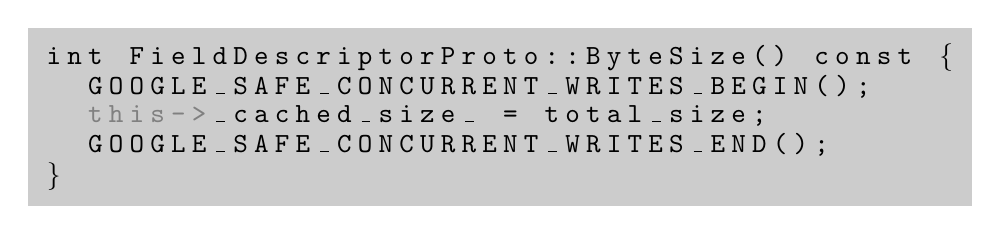
\begin{tikzpicture}
      \matrix {
i \& n \& t \&   \& F \& i \& e \& l \& d \& D \& e \& s \& c \& r \& i \& p \& t \& o \& r \& P \& r \& o \& t \& o \& : \& : \& B \& y \& t \& e \& S \& i \& z \& e \& ( \& ) \&   \& c \& o \& n \& s \& t \&   \& \{ \\
  \&   \& G \& O \& O \& G \& L \& E \& \_ \& S \& A \& F \& E \& \_ \& C \& O \& N \& C \& U \& R \& R \& E \& N \& T \& \_ \& W \& R \& I \& T \& E \& S \& \_ \& B \& E \& G \& I \& N \& ( \& ) \& ; \&   \&   \&   \&   \\
  \&   \& |[black!50]|t \& |[black!50]|h \& |[black!50]|i \& |[black!50]|s \& |[black!50]|- \& |[black!50]|> \& \_ \& c \& a \& c \& h \& e \& d \& \_ \& s \& i \& z \& e \& \_ \&   \& = \&   \& t \& o \& t \& a \& l \& \_ \& s \& i \& z \& e \& ; \&   \&   \&   \&   \&   \&   \&   \&   \&   \\
  \&   \& G \& O \& O \& G \& L \& E \& \_ \& S \& A \& F \& E \& \_ \& C \& O \& N \& C \& U \& R \& R \& E \& N \& T \& \_ \& W \& R \& I \& T \& E \& S \& \_ \& E \& N \& D \& ( \& ) \& ; \&   \&   \&   \&   \&   \&   \\

\} \&   \&   \&   \&   \&   \&   \&   \&   \&   \&   \&   \&   \&   \&   \&   \&   \&   \&   \&   \&   \&   \&   \&   \&   \&   \&   \&   \&   \&   \&   \&   \&   \&   \&   \&   \&   \&   \&   \&   \&   \&   \&   \&   \\
      };
    \end{tikzpicture}
  \end{frame}

  \begin{frame}
    \frametitle{LevelDB's Unique Archetypes}
    \Large
    \begin{tabular}{p{2.65cm} p{4cm} c c}
      \textbf{Root Cause} & \textbf{Main Attribute}
      & \textbf{Not visible?} & \textbf{Synchronized?} \\

      Transitive & Unit Testing & Yes & Yes \\
      Transitive & Buffer/Cache &   & Yes \\
      Transitive & Incorrect &   &   \\
      Transitive & Incorrect &   &   \\
      Transitive & Incorrect &   & Yes \\
      Transitive & Unit Testing & Yes &   \\
    \end{tabular}
  \end{frame}

  \begin{frame}
    \frametitle{LevelDB Not Visible Example}
    \centering
    \large
    
\begin{tikzpicture}
      \matrix  {
 c \& l \& a \& s \& s \&   \& C \& o \& u \& n \& t \& i \& n \& g \& F \& i \& l \& e \&   \& : \&   \& p \& u \& b \& l \& i \& c \&   \& R \& a \& n \& d \& o \& m \& A \& c \& c \& e \& s \& s \& F \& i \& l \& e \&   \& \{ \\

 \&   \& v \& i \& r \& t \& u \& a \& l \&   \& S \& t \& a \& t \& u \& s \&   \& R \& e \& a \& d \& ( \& |[black!50]|. \& |[black!50]|. \& |[black!50]|. \& ) \&   \& |[blue]|c \& |[blue]|o \& |[blue]|n \& |[blue]|s \& |[blue]|t \&   \& \{ \&   \&   \&   \&   \&   \&   \&   \&   \&   \&   \&   \&   \\

  \&   \&   \&   \& |[black!50]|t \& |[black!50]|h \& |[black!50]|i \& |[black!50]|s \& |[black!50]|- \& |[black!50]|> \& c \& o \& u \& n \& t \& e \& r \& \_ \& - \& > \& I \& n \& c \& r \& e \& m \& e \& n \& t \& ( \& ) \& ; \&   \&   \&   \&   \&   \&   \&   \&   \&   \&   \&   \&   \&   \&   \\

  \&   \& \} \&   \&   \&   \&   \&   \&   \&   \&   \&   \&   \&   \&   \&   \&   \&   \&   \&   \&   \&   \&   \&   \&   \&   \&   \&   \&   \&   \&   \&   \&   \&   \&   \&   \&   \&   \&   \&   \&   \&   \&   \&   \&   \&   \\

\} \& ; \&   \&   \&   \&   \&   \&   \&   \&   \&   \&   \&   \&   \&   \&   \&   \&   \&   \&   \&   \&   \&   \&   \&   \&   \&   \&   \&   \&   \&   \&   \&   \&   \&   \&   \&   \&   \&   \&   \&   \&   \&   \&   \&   \&   \\
      };
    \end{tikzpicture}
  \end{frame}

  \begin{frame}
    \frametitle{Unique Archetypes from All Other Projects}
    \Large
    \begin{tabular}{p{2.65cm} p{4cm} c c}
      \textbf{Root Cause} & \textbf{Main Attribute}
      & \textbf{Not visible?} & \textbf{Synchronized?} \\

      \texttt{const\_cast} & Incorrect &   &   \\
      \texttt{mutable} & Incorrect &   &   \\
      \texttt{mutable} & Incorrect &   &   \\
      \texttt{mutable} & Buffer/Cache & Yes &   \\
      \texttt{mutable} & Incorrect &   &   \\
      \texttt{mutable} & Unit Testing & Yes &   \\
    \end{tabular}
  \end{frame}

  \begin{frame}
    \frametitle{fish shell Removes \const{} then Writes}
    \centering
    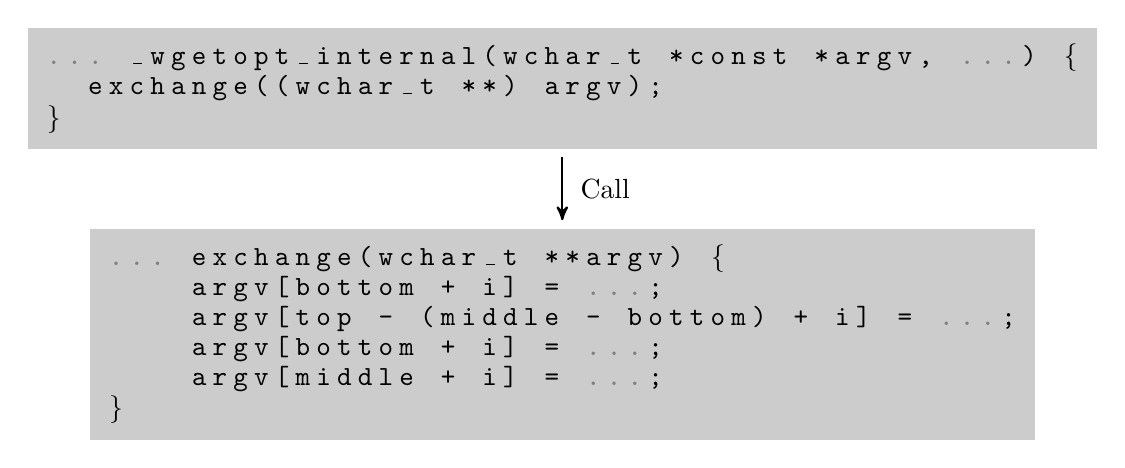
\begin{tikzpicture}

      \matrix (wgetopt) {
|[black!50]|. \& |[black!50]|. \& |[black!50]|. \&   \& \_ \& w \& g \& e \& t \& o \& p \& t \& \_ \& i \& n \& t \& e \& r \& n \& a \& l \& ( \& w \& c \& h \& a \& r \& \_ \& t \&   \& * \& c \& o \& n \& s \& t \&   \& * \& a \& r \& g \& v \& , \&   \& |[black!50]|. \& |[black!50]|. \& |[black!50]|. \& ) \&   \& \{ \\
  \&   \& e \& x \& c \& h \& a \& n \& g \& e \& ( \& ( \& w \& c \& h \& a \& r \& \_ \& t \&   \& * \& * \& ) \&   \& a \& r \& g \& v \& ) \& ; \&   \&   \&   \&   \&   \&   \&   \&   \&   \&   \&   \&   \&   \&    \\
\} \&   \&   \&   \&   \&   \&   \&   \&   \&   \&   \&   \&   \&   \&   \&   \&   \&   \&   \&   \&   \&   \&   \&   \&   \&   \&   \&   \&   \&   \&   \&   \&   \&   \&   \&   \&   \&   \&   \&   \&   \&    \\
  };
      \matrix (exchange) [scale=0.5, below=of wgetopt] {
|[black!50]|. \& |[black!50]|. \& |[black!50]|. \&   \& e \& x \& c \& h \& a \& n \& g \& e \& ( \& w \& c \& h \& a \& r \& \_ \& t \&   \& * \& * \& a \& r \& g \& v \& ) \&   \& \{ \\

  \&   \&   \&   \& a \& r \& g \& v \& \lbrack \& b \& o \& t \& t \& o \& m \&   \& + \&   \& i \& \rbrack \&   \& = \& \& |[black!50]|. \& |[black!50]|. \& |[black!50]|. \& ; \\

  \&   \&   \&   \& a \& r \& g \& v \& \lbrack \& t \& o \& p \&   \& - \&   \& ( \& m \& i \& d \& d \& l \& e \&   \& - \&   \& b \& o \& t \& t \& o \& m \& ) \&   \& + \&   \& i \& \rbrack \&   \& = \& \& |[black!50]|. \& |[black!50]|. \& |[black!50]|. \& ; \\

  \&   \&   \&   \& a \& r \& g \& v \& \lbrack \& b \& o \& t \& t \& o \& m \&   \& + \&   \& i \& \rbrack \&   \& = \&   \&  |[black!50]|. \& |[black!50]|. \& |[black!50]|. \& ; \\

  \&   \&   \&   \& a \& r \& g \& v \& \lbrack \& m \& i \& d \& d \& l \& e \&   \& + \&   \& i \& \rbrack \&   \& = \&   \&  |[black!50]|.\& |[black!50]|. \& |[black!50]|. \& ;   \\

        \} \\
      };

      \draw [arrow] (wgetopt) -- node [right, xshift=1mm] {\normalsize Call} (exchange);
    \end{tikzpicture}
  \end{frame}

  \begin{frame}
    \frametitle{Mosh Writes Directly Through \const{}}
    \centering
    \large
    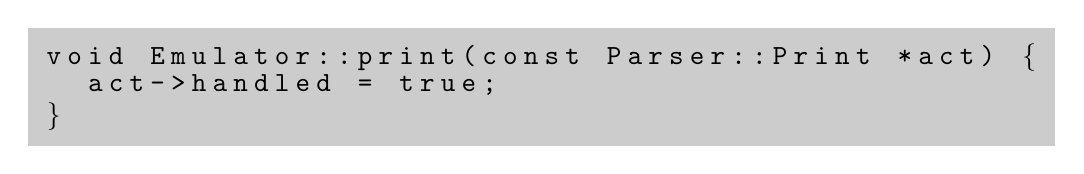
\begin{tikzpicture}
      \matrix  {
v \& o \& i \& d \&   \& E \& m \& u \& l \& a \& t \& o \& r \& : \& : \& p \& r \& i \& n \& t \& ( \& c \& o \& n \& s \& t \&   \& P \& a \& r \& s \& e \& r \& : \& : \& P \& r \& i \& n \& t \&   \& * \& a \& c \& t \& ) \&   \& \{ \\
  \&   \& a \& c \& t \& - \& > \& h \& a \& n \& d \& l \& e \& d \&   \& = \&   \& t \& r \& u \& e \& ; \&   \&   \&   \&   \&   \&   \&   \&   \&   \&   \&   \&   \&   \&   \&   \&   \&   \&   \&   \&   \&   \&   \&   \&   \&   \&   \\
\} \&   \&   \&   \&   \&   \&   \&   \&   \&   \&   \&   \&   \&   \&   \&   \&   \&   \&   \&   \&   \&   \&   \&   \&   \&   \&   \&   \&   \&   \&   \&   \&   \&   \&   \&   \&   \&   \&   \&   \&   \&   \&   \&   \&   \&   \&   \&   \\
      };
    \end{tikzpicture}
  \end{frame}

  \begin{frame}
    \frametitle{Answers to Research Questions}
    \Large
    \begin{enumerate}
      \setlength\itemsep{0.5em}
      \item Developers routinely write-through-\const{}
      \item Equally prefer using \texttt{mutable} and transitive
      \item The majority of the time developers should not write-through-\const{}
    \end{enumerate}
  \end{frame}

  \begin{frame}
    \frametitle{Summary}
    \Large
    Most developers intend to mean deep abstract immutability

    \vspace{1em}
    There are legitimate reasons for \texttt{mutable}

    \vspace{1em}
    Currently, most writes-through-\const{} should not happen
  \end{frame}

  \begin{frame}
    \frametitle{Try It Out}

    \begin{center}
      \includegraphics[scale=0.1]{aec-badge-ecoop}

      \vspace{0.25em}
      \texttt{\huge https://github.com/eyolfson/}
      \texttt{https://github.com/eyolfson/research-2016-ecoop-artifact/}
      \texttt{https://github.com/eyolfson/research-2016-ecoop-paper/}
    \end{center}

  \end{frame}
\end{document}
